\documentclass{article}
\usepackage[utf8]{inputenc}
\usepackage{graphicx}
\graphicspath{ {assets/} }
\usepackage{hyperref}
\usepackage{eurosym}

\renewcommand{\labelitemi}{$\textendash$}

\title{About handling a distributed system using a file system hierarchy [draft]}
\author{Morandini, Daniel \\ \texttt{daniel.morandini@keepinmind.info}}
\date{May 2020}

\begin{document}

\maketitle
\section{Current architecture with systemd and message queues}
We have a server which is taking user requests through an HTTP web interface. Users have the ability to execute some resource-consuming processes through it, such as video transcoding among them, which is an high CPU/GPU usage activity by its nature.
The different function of the web server with respect to the other processors made us naturally build the infrastructure as a set of specific-purpose servers, each with a clear and defined task: the transcoding server, the web server, etc. Each service is deployed separately in a different physical server with the most convenient hardware specs for the task. The services communicate using an asynchronous message queue system. The technology of choice is \textit{RabbitMQ} \footnote{\url{https://www.rabbitmq.com}}. An overview of the setup is shown in figure \ref{fig:1}.
\begin{figure}[h]
    \centering
    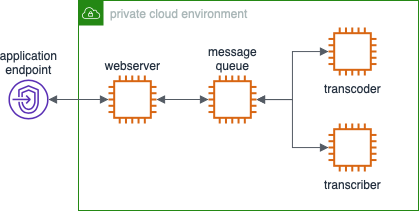
\includegraphics[width=.6\textwidth]{current-cloud.png}
    \caption{Servers composing the current architecture}
    \label{fig:1}
\end{figure}
Even though each service runs in a separate server, it does not mean that it cannot be overwhelmed by the number of task requests, leading to a resource overload. This is why each service has a configurable number of parallel instances that is allowed to run to complete the requested tasks. Those numbers were obtained by overloading the servers on purpose.

The services run as \textit{systemd} \footnote{\url{https://en.wikipedia.org/w/index.php?title=Systemd&oldid=955047185}} supervised processes. Each service is wrapped around a library that we reuse for establishing the queue connection, bounding the process concurrency and using a homogeneous policy for message acknowledgements (we do not want to loose messages when failures occur).

We deploy the services using custom \textit{Ansible} \footnote{\url{https://www.ansible.com}} scripts. Each time we release a new version of a service, it is tagged, built, its artifacts uploaded in an \textit{AWS S3} bucket and eventually downloaded and run in the targeted servers.

The above infrastructure performs quite well in terms of maintainability and reliability when the number of customers accessing the platform is stable, which was the case in the early stages of the product. Now we are facing a usage increment, and we are aware that, if not addressed, this configuration will arise the following - non exhaustive - list of issues

\begin{enumerate}
    \item we do speech to subtitles transcription of live video transmissions. The number of concurrent transcribers that can run is upper bounded, which means that \textbf{if a user requests a transcription in the wrong (or right, one might say) moment, the service will not be available}. We want to address this issue by increasing the number of service processes on demand.
    \item Transcoding requires high performance hardware do deliver the results to the users in a meaningful time. The \textit{AWS g3s.xlarge} server instance types suite our needs, with a cost of \textit{\$0.796/hour}, or roughly \textit{\EUR{500}/month}. We handle up to four concurrent tasks on each of these instances, but most of the time they sit there idle. We want to be capable of shutting those kind of servers down when we do not need them, to \textbf{save energy and money}.
\end{enumerate}

This configuration does not address very gracefully another issue too not related to the usage increment stated above. Each service runs as an always on daemon. When a code update is performed, servers need to be taken down and up again with the new version. In our case, we need the live transcribers to terminate their sub-processes (some live-streams last up to six hours) before shutting them down. This is why we would rather have a process spawned for each task, picking the latest version of the software needed each time. The task comes in, a process is spawned for it and starts the execution: when complete, the process is terminated. Updates never stop running daemons.

\section{About the new solution}
The new infrastructure should introduce a single always-running component which responsibility is to collect tasks and spawn a dedicated process (more on this later) for each one of them, dynamically. 
This setup allows the dispatcher to make some useful decisions at run-time, like picking the preferred version of the software to use for solving the task. This way we avoid the upgrading problems \textbf{by bounding the software's life-cycle to its task}.

Up to now we delivered tools as native binary executables (cross-compiled using \textit{Go} \footnote{\url{https://golang.org}}), which (only in the transcoders case) have a single run-time dependency, \textit{ffmpeg} \footnote{\url{https://ffmpeg.org}}. The packaging and distribution complexity is hence reduced, but we don't want to develop a solution that is language dependent, nor one that does not gracefully manage a greater number of run-time dependencies. \textit{OS-level virtualization} \footnote{\url{https://en.wikipedia.org/w/index.php?title=OS-level_virtualization\&oldid=948517170}} is the state-of-the-art approach for coping with this kind requirements: the software is distributed together with its run-time environment, making the most intricate system easy to deploy and execute outside of its development context.

With this configuration, we increase the flexibility of the task dispatcher lowering its complexity and simplifying its task: executing software images on the most appropriate hardware.

While the task is being executed, a mechanism for accessing status updates, error conditions and return values should be provided to the clients. The solution should hide the complexity of accessing these information with a large number of tasks running concurrently.

\subsection{Implementation details: 9p, fargate}
Using the \textit{9p protocol}\footnote{\url{http://doc.cat-v.org/plan_9/misc/ubiquitous_fileserver/}}, developed for the distributed operating system \textit{Plan9}\footnote{\url{https://plan9.io/plan9/}} at Bell Labs, we present a file system hierarchy that allows to interact with our solution. Our servers and developers (while debugging or developing), can \texit{mount}\footnote{\url{http://man.cat-v.org/plan_9/1/bind}} a remote process on their file system, allowing them to interact with it through its virtual files. The API for interacting with the system is provided through the basic read/write operations performed on what appear to be regular files.

Software is distributed as \textit{Docker} \footnote{\url{https://www.docker.com}} \texit{images}, which can be executed on each machine that is running a docker daemon. An image is a self-contained environment for our service to run, ships without any external dependency with the exception of the docker daemon. With this configuration, we obtained a well defined differentiation between the services themselves and the actual environment hosting the \textit{containers} (images at execution-time), leading to a greater division of concerns: on one side the code with its dependencies, on the other the management of the container distribution, i.e. hardware resource management.

The task dispatcher only has to ask for a container to a docker daemon, which in turn could have at its disposal a set of machines that might run the selected image. In our case, we selected as starting point \textit{AWS Fargate} \footnote{\url{https://aws.amazon.com/fargate/}} as container management infrastructure. Based on the task, the container is run on the most appropriate host environment, in terms of performance capabilities. This vendor-locking dependency may be dropped at will, as the solution is flexible enough to allow us to migrate to any kind of container management environment, e.g. a self-hosted \textit{Kubernetes} \footnote{\url{https://kubernetes.io}} or \textit{Docker Swarm} \footnote{\url{https://docs.docker.com/engine/swarm/}} cluster.

\subsection{Flexi}
This section makes a walk-through of the implementation details of the solution under development. The source code is available on \textit{Github}, under the \textit{flexi}\footnote{\url{https://github.com/jecoz/flexi}} repository. The discussion in based on the progress made up to version \textit{v0.1.1}\footnote{\url{https://github.com/jecoz/flexi/tree/v0.1.1}}.

Figure \ref{fig:fsh} shows how the flexi file system would look like after a successful mount, in this case presenting two processes still under use.
\begin{figure}[h]
    \centering
    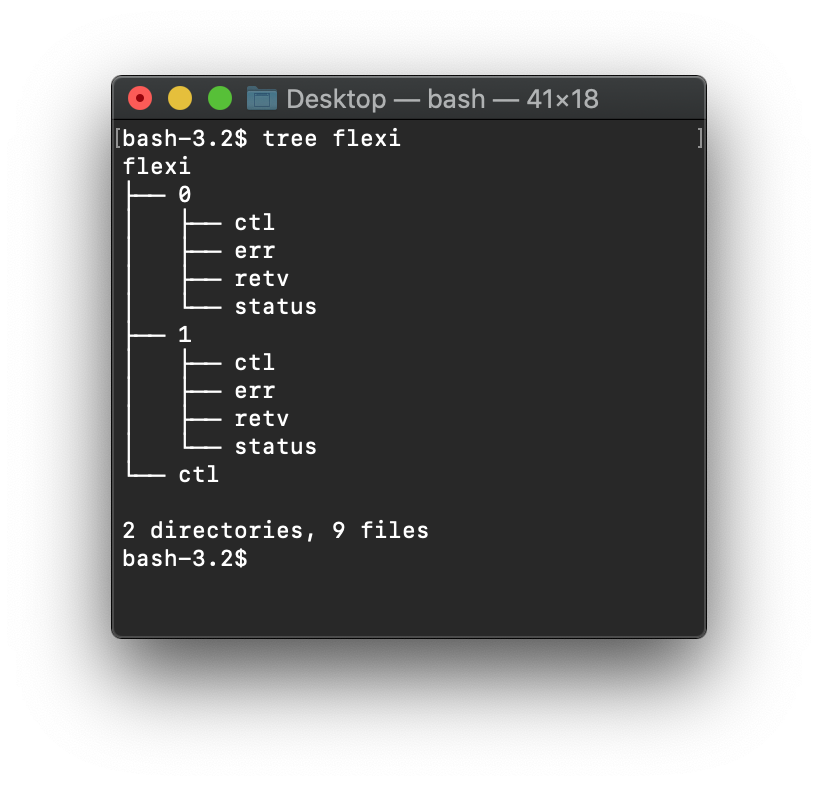
\includegraphics[width=.7\textwidth]{flexi-tree.fake.1.png}
    \caption{File system hierarchy of a flexi folder, with two processes.}
    \label{fig:fsh}
\end{figure}

The idea is that to start a new process, a user writes a JSON encoded task \footnote{An example file can be found at \url{https://github.com/jecoz/flexi/blob/17f6ca1baa1478d3d8b66350c02f2f15c2d4045a/testdata/input.1.json}} in the flexi/ctl file. At this point flexi spawns a container on a machine that fulfills the required hardware capabilities for that task, obtains the public IP address of the container and mounts it locally under a sequentially indexed directory, lets assume number 3. This first stage starts the container, the client can then write the input data (that might be different depending on the image) in the flexi/3/ctl file, and read the output produced from the flexi/3/err and flexi/3/retv files, containing errors (if any) and return value, respectively.

The v0.1.1 of flexi does not yet provide the whole file system hierarchy, but only the libray code written in Go that allows to write a process that serves a 9p server exposing the ctl, err and retv files, together with some useful helpers.

Under examples/, \textit{echo64spawner} allows to spawn the \textit{echo64} Docker image on fargate \footnote{which "task definition" has to be predefined on the AWS console, see \url{https://github.com/jecoz/flexi/blob/3a823b1f6e31e04c890db8feeec201c1dcd19003/testdata/echo64.taskdefinition.ecs.json}}. If successful, the executable returns a JSON encoded "remote process" structure, which contains the public IP address of the container. The client can mount the container locally as described above, play with it and eventually "umount" the resource.

\textit{echo64killer} takes as input the JSON payload returned by echo64spawner and stops the container.

\section{Notes}
\subsection{AWS server-less technologies (i.e. Lambda) do not fit well as they are implemented}
Readers might think about leveraging \textit{AWS Lambda} \footnote{\url{https://aws.amazon.com/lambda/}} server-less solution to solve this kind of scalability issues. While bringing advantages on one side, it makes it more difficult to cope with other critical aspects of the software system we're building: some services require to expose endpoints over the Internet, such as the live transcoders and transcribers. While running, they read a stream of bytes from a TCP port \textbf{previously selected in coordination with the web server}, which must now this information before starting the live-streaming pipeline. This task is not easily accomplished within lambda's context. Another drawback is hardware capabilities selection. For transcoding we need to be able to choose the GPU that will be available within the container, even though we do not care \textbf{which machine is eventually picked}, as long as these requirements a met. At the time of writing, this is another feature not available if using lambdas. Finally, the live transcription tasks may last more than 6 hours long, which make lambda's pricing model less convenient for our use-case.

\end{document}
